\section{MM TP Algorithm}
\label{sec:alg}

The MM TP algorithm is designed to receive ART data from the ADDC, decode the data, group the data into subsets (``triggers'') which satisfy a spatial and temporal coincidence, and calculate quantities which describe these triggers. The first step is referred to as the \textit{decoder}, the second step is referred to as the \textit{finder}, and the third step is referred to as the \textit{fitter}.

The MM TP algorithm is written in firmware and placed on a Xilinx Virtex-7 FPGA, which is housed by a VC707 evaluation board. The algorithm meets timing requirements for synthesis and implementation of the algorithm on the FPGA. Ultimately, the algorithm will be placed on a larger FPGA on a high-density optical mezzanine card (``HORX'') which will be housed in an ATCA shelf. The VC707 implementation is already capable of testing many aspects of the algorithm, however, including the steps mentioned above.

\subsection{Decoding}
\label{sec:alg-decode}

ART data is transmitted from the ADDC to the MM TP using the GBT protocol via optical fibers. The data is transmitted as one 128-bit word per BC per ADDC. 12 bits describe the BCID; 32 bits describe which of the 32 VMMs associated with one ADDC are transmitting an ART signal; 48 bits give a maximum of 8 ART strip numbers, which are 6 bits each; and the remaining bits are used for checking data quality, such as an 8-bit data parity word.

After receiving the ART data, the MM TP converts the VMM and strip numbers into global strip numbers, also taking into consideration that some of the MM chambers are flipped relative to each other. For example, if an ART strip from VMM 5 is reported as strip number 30, the MM TP converts this to a global strip number of 350 ($5*64 + 30$). The units of the MM TP are strip pitches, and there is no conversion to a unit of meters. The MM TP then adds the distance from the beamline to the base of the MM chamber, in units of strips, to the global strip number, and divides the global strip number by the $z$-position of the chamber, to convert the strip to a slope, $x_\text{strip} / z_\text{strip}$.

\subsection{Adjustments for cosmic muons}
\label{sec:alg-crts}

The use of \textit{slopes} instead of \textit{strips} is motivated by the knowledge that particles arriving at the NSW from a proton-proton collision should travel in a nearly straight line. Thus, each layer of MM will record a different strip address for the incident particle, but a nearly identical slope. This simplifies logic for defining spatial \textit{roads} in the MM chamber.

However, for a cosmic ray test stand, the exact origin of incident particles is unknown. The MM TP algorithm is then modified to use strip addresses instead of slopes for the defintion of roads, as discussed in Section~\ref{sec:alg-finder}. The implementation of strip-to-slope conversion in the FPGA is nonetheless tested by multiplying each strip address by 1, instead of $1/z_\text{strip}$, to calculate a ``slope'' which is suitable for spatial coincidences of cosmic muons.

Additional adjustments to the MM TP algorithm for use at the cosmic ray test stand include: \textbf{PUT ADJUSTMENTS HERE}

\subsection{Finder}
\label{sec:alg-finder}

Once the ART data is received and decoded, the next step of the MM TP algorithm is to filter the data into subsets which roughly look like an incident particle traversing the octuplet. This step is called the \textit{finder}.

The finder relies heavily on parallelization. A configurable number of roads are created in the FPGA to span the octuplet, and each roads evaluates in parallel whether is contains a sufficient number of ART strips to form a trigger. In this note, the road size is 1 road per VMM. This is demonstrated graphically in Figure~\ref{}.

Additionally, the roads should overlap to avoid edges cases where the incident muon travels near to the boundary of two roads. This is implemented in the finder by allowing each road to use hits not only in their respective road, but also in neighboring roads. The number of neighboring roads is a configurable parameter; in this note, hits from one neighbor above and one neighbor below are used in a given road. For example, road 3 uses hits from VMM 2, VMM 3, and VMM 4, so that the effective road size is 3 VMMs.

The effective road size is chosen to balance the acceptance of cosmic ray muons in the octuplet, the acceptance of the scintillator triggers, and the rejection of background hits. The incident angle of cosmic muons is shown in previous studies with this detector~\ref{}, which is at most 25 degrees. Muons with an angle of 26 degrees can be observed with an effective road size of 3 VMMs, as shown in Figure~\ref{fig:cartoon_road_efficiency}, though some inefficiency can be expected starting at 18 degrees, depending on the position of the muon.

\begin{figure}[!htpb]
  \begin{center}
    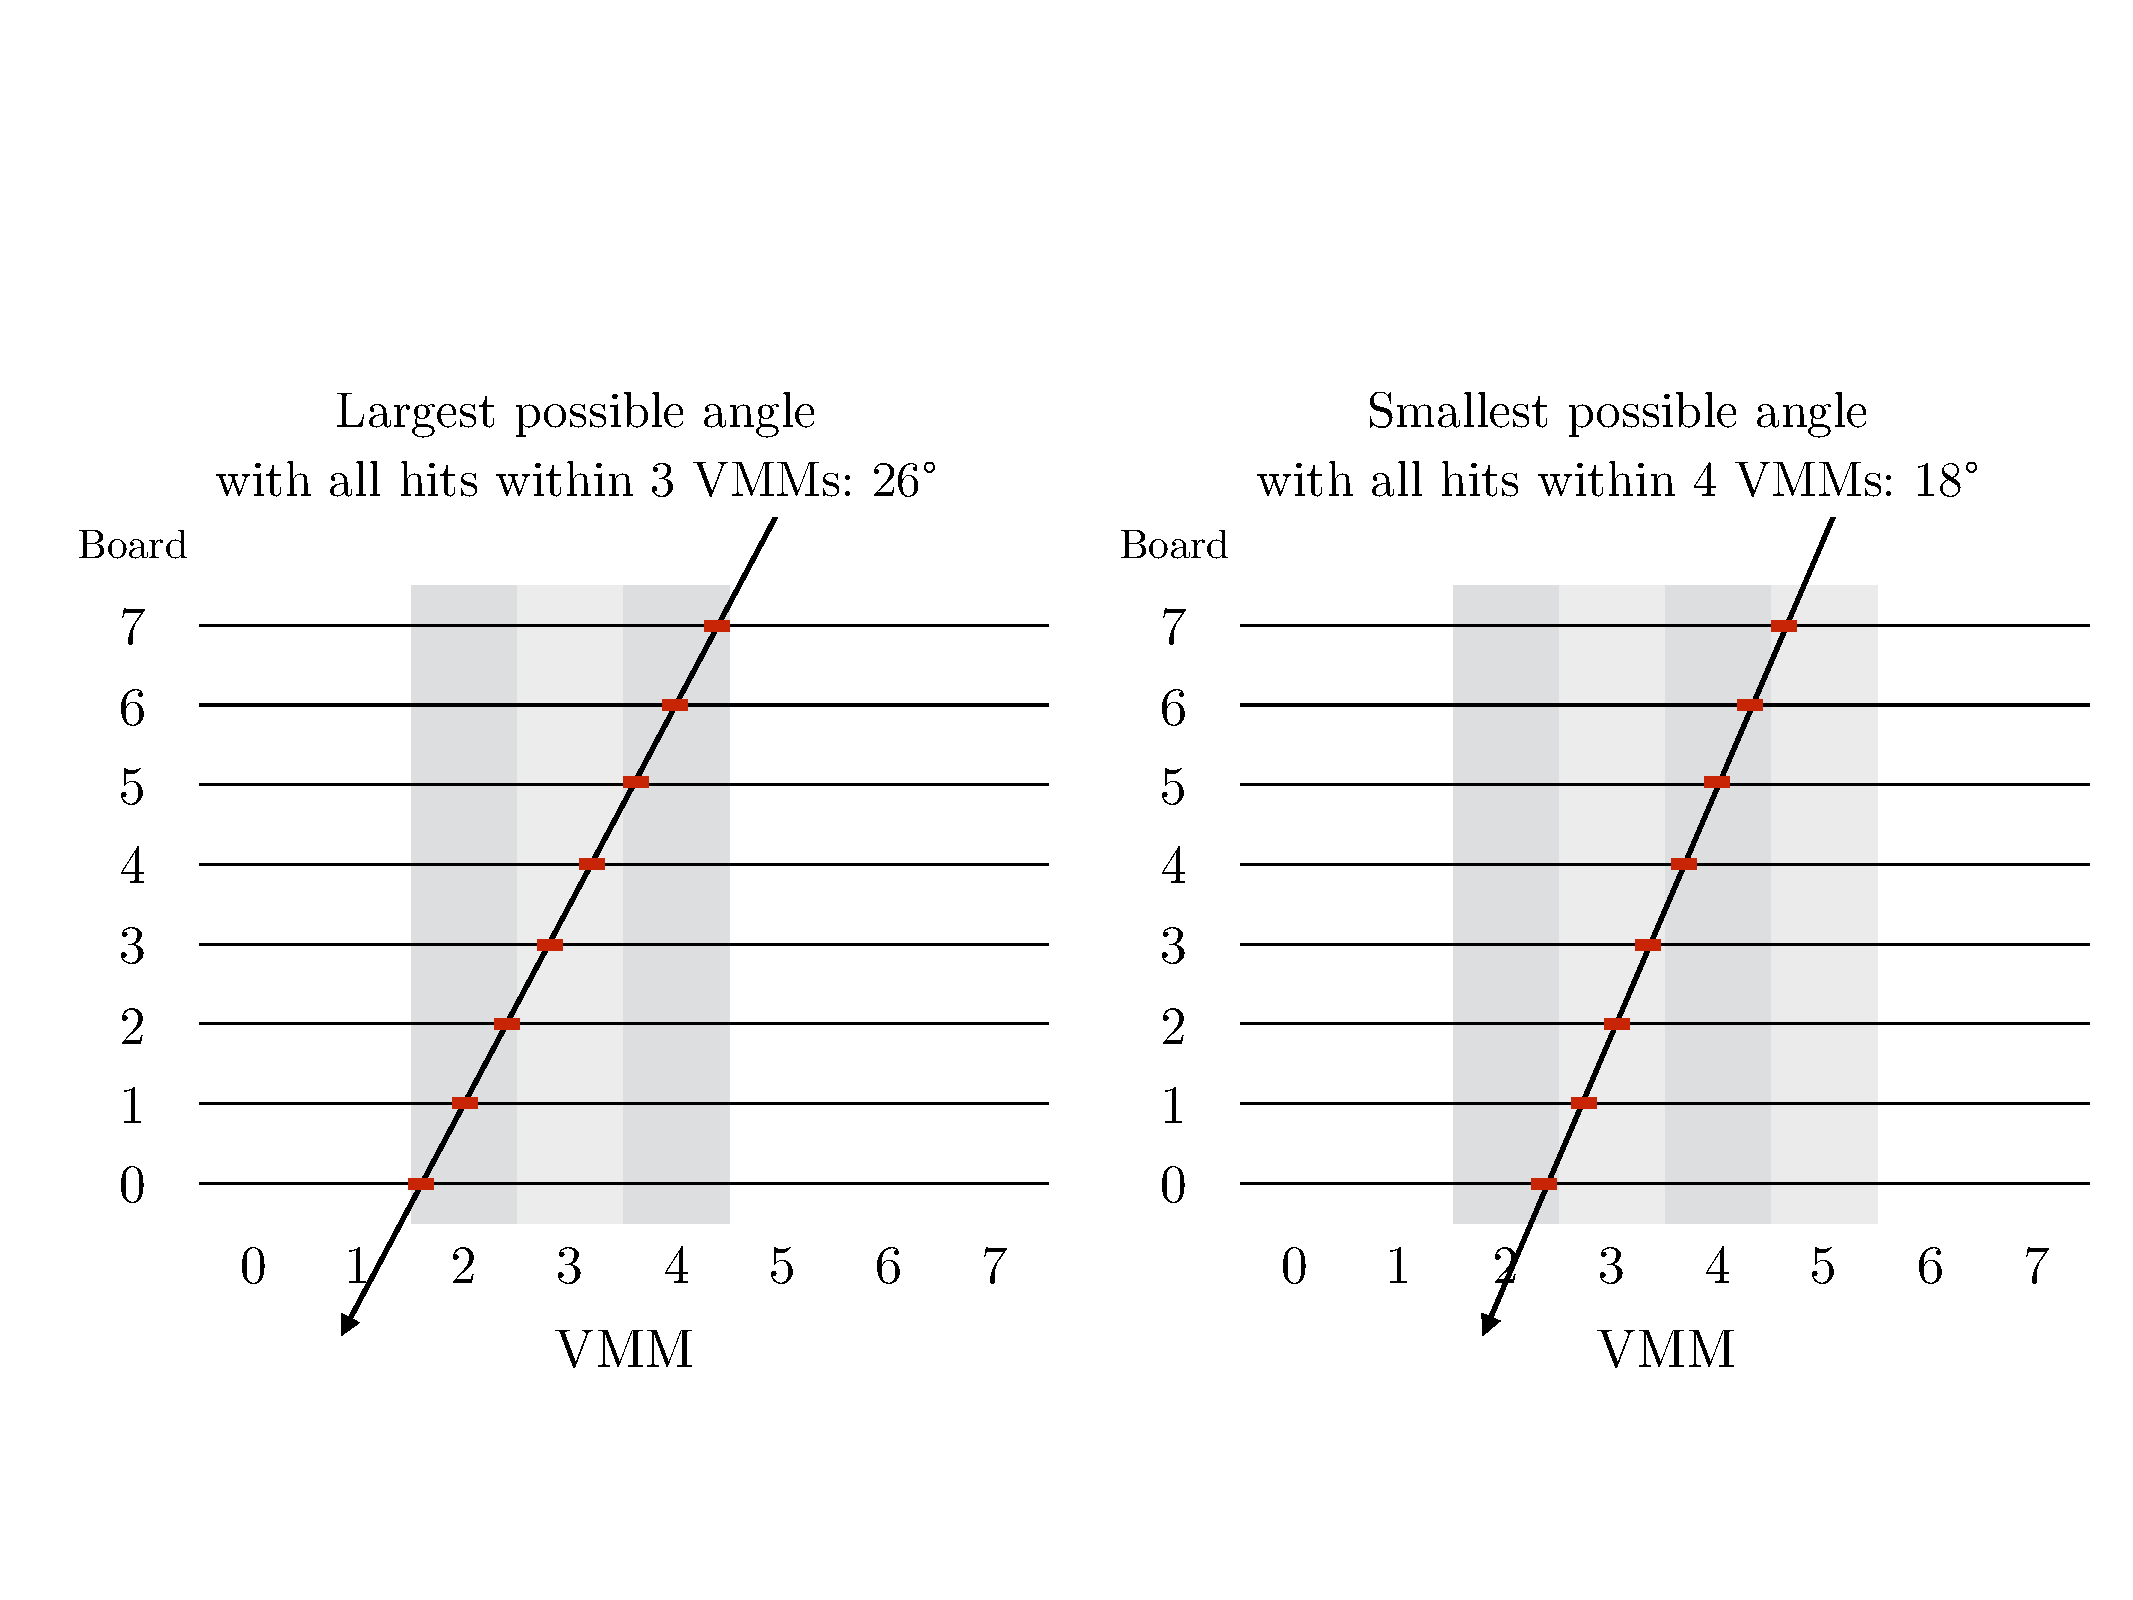
\includegraphics[width=1.0\textwidth]{figures/cartoons/cartoon_road_efficiency}
  \end{center}
  \vspace{-20pt}
  \caption{Cartoon demonstration of the highest-angle track with all 8 hits spread across 3 VMMs (left) and the lowest-angle track with at least one hit spread across 4 VMMs (right). The angles are 26 and 18 degrees, respectively. An effective road size of 3 VMMs should then have 100\% hit efficiency up to 18 degrees.}
  \label{fig:cartoon_road_efficiency}
\end{figure}

A road must contain at least two hits on horizontal ($X$) planes and at least two hits on stereo ($UV$) planes to be satisfy a trigger. Additionally, at least two of the hits on $X$-planes must occur on opposite quadruplets, to ensure a good lever arm when fitting the $X$-hits to a line. These requirements are looser than the expected coincidence requirements at the NSW ($3X$ AND $3UV$), since the rate of noise and background hits is much lower for cosmic data-taking than at the LHC.

The finder also requires hits for a trigger to be within a time window in units of the BC clock. The expected time window for the NSW is two BCs; in this note, the window is increased to seven BCs to maximize efficiency and measure the efficiency of the window as a function of the size of the window. The time window is implemented as follows. When a hit arrives at the finder, it is stored in memory for seven BCs. For each road satisfied by the hit, no new hits are allowed in that road for that board until the hit is ``old'', i.e., after seven BCs. As hits are recorded, the coincidence requirements are evaluated for all roads in parallel. Once the coincidence requirements for a road are met and the earliest hit in the road becomes ``old'', a trigger is formed. Therefore hits are collected in a time window of seven BCs, and triggers cannot be formed until the oldest hit in the road is sufficiently old.

The stipulation that a hit in a road on a board cannot be overwritten by a new hit is motivated by the behavior of the detector and the ART data-flow: an incident muon is expected to leave a signal on multiple strips on a board (making a ``cluster''), each strip of which can send an ART signal typically separated by a couple of BCs. Only the first hit from the cluster should be used for the trigger, hence the earlier hit should not be overwritten by subsequent nearby hits. 

Every road is capable of forming one trigger per cycle of the BC clock. After evaluating all roads in parallel, the triggers created are placed in a priority encoder to be sent sequentially to the fitter for further calculations. The priority encoder sorts the triggers by road number, with smallest roads treated first. Because the MM TP clock is eight times faster than the BC clock, there can be at most eight triggers per BC.

\subsection{Fitter}
\label{sec:alg-fitter}

The triggers found by the finder are then sent to the \textit{fitter}, which calculates quantities of interest for the trigger. The fitter does not create or remove any triggers. The NSW implementation of the fitter is described first, and modifications for cosmic data-taking are described second.

For the NSW, the main deliverables of the fitter are the location and quality of a trigger. The location is represented by a region of interest (ROI), which is a number provided by downstream clients like Sector Logic mapping to $\eta-\phi$ space. The quality of the trigger is represented by the difference in angle a \textit{local} fit of the trigger ART hits and a \textit{global} fit. A \textit{local} fit is performed on only the ART hits, and a \textit{global} fit is performed with the constraint that the trigger be consistent with the interaction point.

The location of the trigger is derived in a Cartesian $m_x-m_y$ space, where $\hat{y}$ points perpendicular to the direction of the $X$-strips, $\hat{x}$ points parallel to the $X$-strips, and $m_i$ is the slope $i/z$\footnote{We apologize for the confusing notation. To recap: $X$, $U$, and $V$ denote different layers of micromegas. $x$, $y$, and $z$ are cartesian coordinates. The $X$-layers measure $m_y$.}. $m_y$ is measured as the average of slopes measured in each $X$-plane, $\overline{m_X}$. $m_x$ is measured as the difference between slopes measured in the $U$ and $V$ planes, with a geometric factor from the angle of the stereo strips: $\frac{m_U - m_V}{2\ \text{tan}(\theta_\text{stereo})}$.

\subsection{Output}
\label{sec:alg-output}

Finally, the MM TP algorithm stores copies of the input ART data and output trigger data in FIFO buffers, which are transmitted as UDP packets via ethernet to a computer for analysis.

\subsection{Bugs encountered}
\label{sec:alg-bugs}

By January 2017, the MM TP algorithm had been implemented in firmware and successfully created triggers in behavioral simulation. By summer 2017, the MM TP algorithm is implemented on a FPGA and records hundreds of thousands of cosmic muon triggers per day. Many bugs were uncovered along the way.


